% ============================================================
% CAPÍTULO 3: FORMULAÇÃO DO PROBLEMA E MODELAGEM DO SISTEMA
% ============================================================
\section{Formulação do Problema e Modelagem do Sistema}
\label{sec:problem_formulation}

Para analisar o comportamento do EKF quanto à convergência, ajuste de parâmetros e consistência estatística, este estudo delineia um cenário de rastreamento bidimensional baseado exclusivamente em dados de distância (\textit{range-only tracking}) \cite{barshalom2001estimation}. Essa modelagem expande o método sugerido em \cite{falek2020computer}, descrevendo a movimentação do agente por meio de um modelo cinemático estruturado no espaço de estados de Posição, Velocidade e Aceleração (PVA).

\subsection{Descrição do Problema}
\label{subsec:problem_description}

O problema abordado consiste em estimar a trajetória de um robô móvel que opera em um plano bidimensional. O agente se desloca dentro de uma arena monitorada por uma infraestrutura de localização local, composta por $M = 4$ estações fixas (âncoras) instaladas em posições conhecidas, denotadas por $\mathbf{p}_i = [X_i, Y_i]^T$ para $i = 1, \dots, 4$. O arranjo completo desse ambiente operacional encontra-se esquematizado na Figura \ref{fig:diagrama_multilateracao}. 

O robô não possui sensores de odometria ou de velocidade própria, dependendo exclusivamente de medições escalares de distância obtidas via radiofrequência ou ondas acústicas em relação a cada uma das estações. O objetivo do estimador é processar essas observações ruidosas e reconstruir, a cada passo temporal, a posição horizontal ($X$) e vertical ($Y$) do agente, estimando também suas componentes de velocidade e aceleração instantâneas.

\begin{figure}[h]
    \centering
    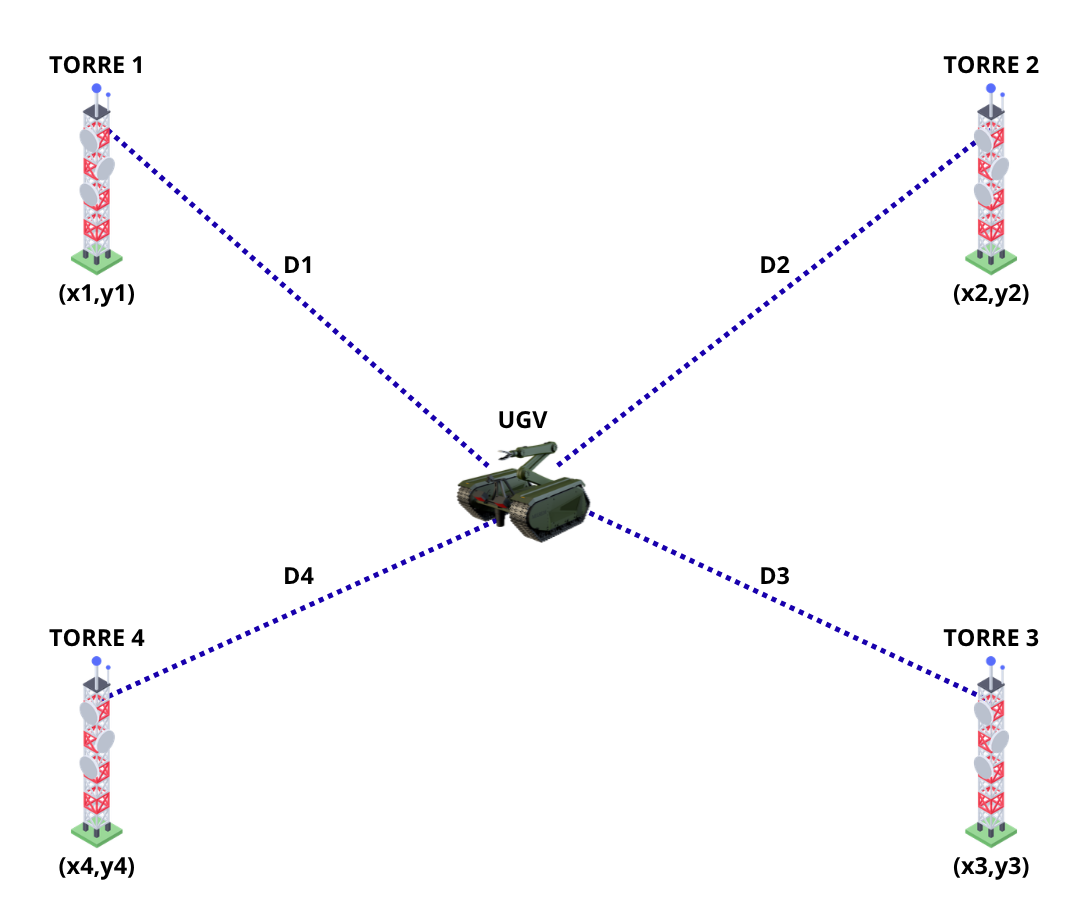
\includegraphics[width=0.5\textwidth]{Figuras/diagrams/MULTILATERAÇÃO.png}
    \caption{Representação geométrica do sistema de posicionamento: o agente móvel no espaço bidimensional e os raios de medição (\textit{range-only}) oriundos das quatro estações base fixas nos vértices da arena.}
    \label{fig:diagrama_multilateracao}
\end{figure}


\subsection{Modelo Cinemático de Processo (Espaço de Estados PVA)}
\label{subsec:pva_model}

Diferentemente de abordagens simplificadas de velocidade constante, o estado do agente móvel no instante discreto $k$ passa a ser representado por um vetor expandido de seis dimensões: $\mathbf{x}_k = [x_k, y_k, v_{x,k}, v_{y,k}, a_{x,k}, a_{y,k}]^T$. Nessa estrutura, $(x_k, y_k)$ correspondem às coordenadas de posição cartesiana, $(v_{x,k}, v_{y,k})$ às componentes da velocidade linear e $(a_{x,k}, a_{y,k})$ às acelerações instantâneas nos eixos $X$ e $Y$, respectivamente.

A dinâmica temporal do sistema sob regime de aceleração constante (CA) é integrada ao longo do intervalo de amostragem $\Delta t$. Essa operação dá origem à matriz de transição de estados $\mathbf{A}_k$ ($6 \times 6$), especificada na Equação (\ref{eq:matriz_A_pva}):

\begin{equation}
    \label{eq:matriz_A_pva}
    \mathbf{A}_k = \begin{bmatrix} 
    1 & 0 & \Delta t & 0 & \frac{\Delta t^2}{2} & 0 \\ 
    0 & 1 & 0 & \Delta t & 0 & \frac{\Delta t^2}{2} \\ 
    0 & 0 & 1 & 0 & \Delta t & 0 \\ 
    0 & 0 & 0 & 1 & 0 & \Delta t \\ 
    0 & 0 & 0 & 0 & 1 & 0 \\ 
    0 & 0 & 0 & 0 & 0 & 1 
    \end{bmatrix}
\end{equation}

Fatores práticos como o escorregamento de rodas, desalinhamentos mecânicos e irregularidades do terreno introduzem erros cumulativos na navegação \cite{thrun2005probabilistic}. Na formulação PVA escolhida, esse comportamento estocástico é transposto para o modelo admitindo que as perturbações ajam de forma independente sobre os componentes de posição, velocidade e aceleração. Essas fontes de incerteza são sintetizadas pela matriz de densidade espectral de potência contínua $\mathbf{Q}_c = \text{diag}(q_1, q_2, q_3, q_4, q_5, q_6)$. 

Ao calcular a discretização analítica desse termo, ponderada pela própria dinâmica veicular no intervalo $\Delta t$, obtém-se uma matriz de covariância discreta $\mathbf{Q}_k$ caracterizada por ser esparsa e simétrica. O perfil estritamente diagonal de $\mathbf{Q}_c$ garante o desacoplamento estocástico entre as dinâmicas dos eixos horizontal ($X$) e vertical ($Y$). Os elementos não nulos associados aos estados do eixo X (índices 0, 2 e 4) são calculados conforme as relações dispostas na Equação (\ref{eq:matriz_Q_pva_x}):

\begin{equation}
    \label{eq:matriz_Q_pva_x}
    \begin{cases}
        Q_{0,0} = q_1\Delta t + q_3\frac{\Delta t^3}{3} + q_5\frac{\Delta t^5}{20} \\
        Q_{0,2} = Q_{2,0} = q_3\frac{\Delta t^2}{2} + q_5\frac{\Delta t^4}{8} \\
        Q_{0,4} = Q_{4,0} = q_5\frac{\Delta t^3}{6} \\
        Q_{2,2} = q_3\Delta t + q_5\frac{\Delta t^3}{3} \\
        Q_{2,4} = Q_{4,2} = q_5\frac{\Delta t^2}{2} \\
        Q_{4,4} = q_5\Delta t
    \end{cases}
\end{equation}

De maneira análoga, os componentes vinculados ao eixo Y (índices 1, 3 e 5) replicam essa mesma estrutura algébrica, utilizando as variâncias espectrais específicas $\{q_2, q_4, q_6\}$ detalhadas na Equação (\ref{eq:matriz_Q_pva_y}):

\begin{equation}
    \label{eq:matriz_Q_pva_y}
    \begin{cases}
        Q_{1,1} = q_2\Delta t + q_4\frac{\Delta t^3}{3} + q_6\frac{\Delta t^5}{20} \\
        Q_{1,3} = Q_{3,1} = q_4\frac{\Delta t^2}{2} + q_6\frac{\Delta t^4}{8} \\
        Q_{1,5} = Q_{5,1} = q_6\frac{\Delta t^3}{6} \\
        Q_{3,3} = q_4\Delta t + q_6\frac{\Delta t^3}{3} \\
        Q_{3,5} = Q_{5,3} = q_6\frac{\Delta t^2}{2} \\
        Q_{5,5} = q_6\Delta t
    \end{cases}
\end{equation}


\subsection{Modelo de Observação e Geometria das Estações Base}
\label{subsec:observation_model}

A partir do arranjo de infraestrutura detalhado na Seção \ref{subsec:problem_description}, o vetor de observações obtido a cada passo amostral é estruturado como $\mathbf{z}_k = [z_{1,k}, z_{2,k}, z_{3,k}, z_{4,k}]^T$. A relação geométrica entre o estado cinemático estimado do robô e a distância escalar real até a $i$-ésima estação fixa é governada por uma função de observação não linear $h_i(\mathbf{x}_k)$, descrita na Equação (\ref{eq:modelo_distancia_nao_linear}):

\begin{equation}
    \label{eq:modelo_distancia_nao_linear}
    h_i(\mathbf{x}_k) = \sqrt{(x_k - X_i)^2 + (y_k - Y_i)^2}
\end{equation}

Como o vetor de estado possui seis dimensões e as leituras dependem estritamente das coordenadas de posição $(x_k, y_k)$, as derivadas parciais da função de medição associadas aos componentes de velocidade e aceleração anulam-se por completo \cite{barshalom2001estimation}. Sob essas condições, a matriz Jacobiana $\mathbf{H}_k$ ($4 \times 6$) avaliada a cada iteração assume o formato estabelecido na Equação (\ref{eq:jacobiano_implementado}):

\begin{equation}
    \label{eq:jacobiano_implementado}
    \mathbf{H}_k = \begin{bmatrix} 
    \frac{x_k - X_1}{h_1(\mathbf{x}_k)} & \frac{y_k - Y_1}{h_1(\mathbf{x}_k)} & 0 & 0 & 0 & 0 \\ 
    \vdots & \vdots & \vdots & \vdots & \vdots & \vdots \\ 
    \frac{x_k - X_4}{h_4(\mathbf{x}_k)} & \frac{y_k - Y_4}{h_4(\mathbf{x}_k)} & 0 & 0 & 0 & 0 
    \end{bmatrix}_{\mathbf{x}_k = \hat{\mathbf{x}}_{k|k-1}}
\end{equation}

Para concluir a modelagem matemática do sensor, a matriz de covariância do ruído de medição é definida como $\mathbf{R}_k = \text{diag}(\sigma_1^2, \sigma_2^2, \sigma_3^2, \sigma_4^2)$, em que cada termo diagonal reflete a variância do erro instrumental intrínseco de sua respectiva âncora de leitura.


\subsection{Cenário de Desafio: Modelagem de Oclusão Temporal}
\label{subsec:occlusion_challenge}

Para avaliar os limites do estimador e a utilidade prática da região de interesse (ROI) dinâmica e do teste NIS, projetou-se uma janela de oclusão severa no ambiente de simulação. Dentro de um intervalo cronometrado $t \in [t_{\text{start}}, t_{\text{end}}]$, as leituras vindas das quatro estações base são intencionalmente suprimidas ($\mathbf{z}_{i,k} \to \emptyset$).

Esse bloqueio — cujo comportamento é ilustrado na Figura \ref{fig:comportamento_elipses} — força o algoritmo a depender apenas das projeções geradas pela matriz de transição PVA (\ref{eq:matriz_A_pva}). Sob condições normais de operação com o filtro atualizando as medições, a elipse mantém-se estável e restrita (Figura \ref{fig:elipse_estavel}). Contudo, sem o suporte das correções trazidas pelos sensores durante a oclusão, as incertezas de aceleração modeladas em $\mathbf{Q}_k$ acumulam-se rapidamente. O resultado direto é uma expansão geométrica acentuada na matriz de covariância predita ($\mathbf{P}_{k|k-1}$), que se traduz no alargamento progressivo da elipse de confiança (ROI) ao longo do deslocamento do robô, variando conforme a trajetória realizada (Figuras \ref{fig:elipse_crescente_1} e \ref{fig:elipse_crescente_2}).


\begin{figure*}[t!]
    \centering
    
    % Subfigura A: Filtro atualizando / Comportamento estável
    \begin{subfigure}[b]{0.32\textwidth}
        \centering
        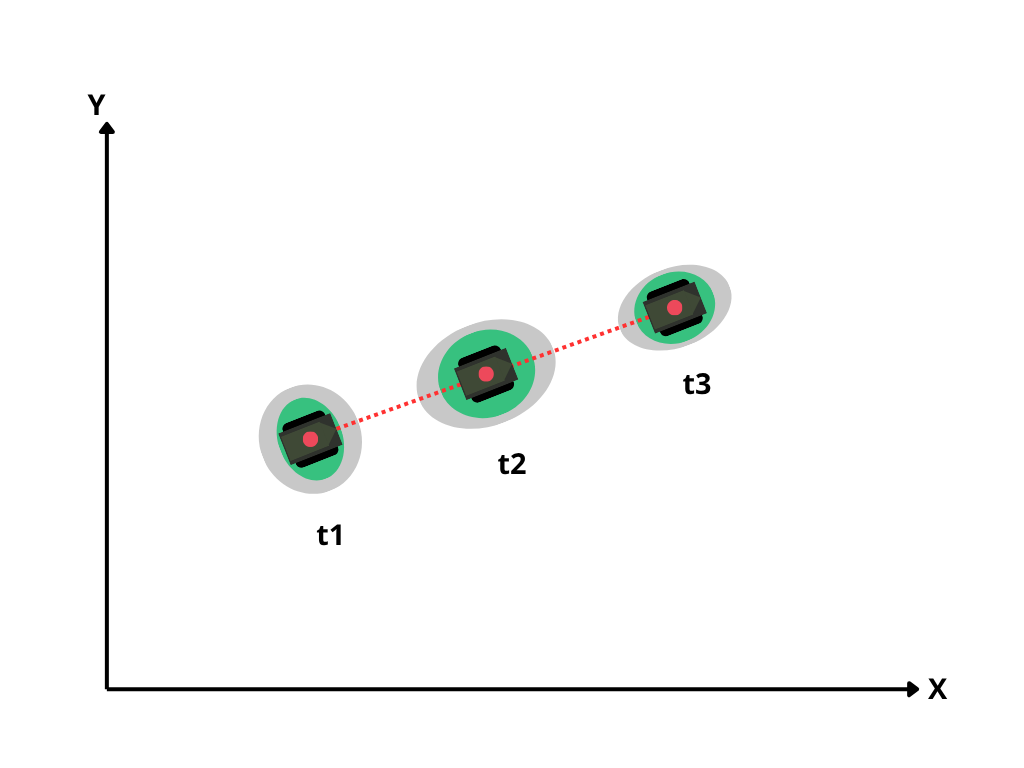
\includegraphics[width=\linewidth]{Figuras/diagrams/PREVISAO.png}
        \caption{Operação nominal: predição e atualização.}
        \label{fig:elipse_estavel}
    \end{subfigure}
    \hfill
    % Subfigura B: Crescimento na trajetória 1
    \begin{subfigure}[b]{0.32\textwidth}
        \centering
        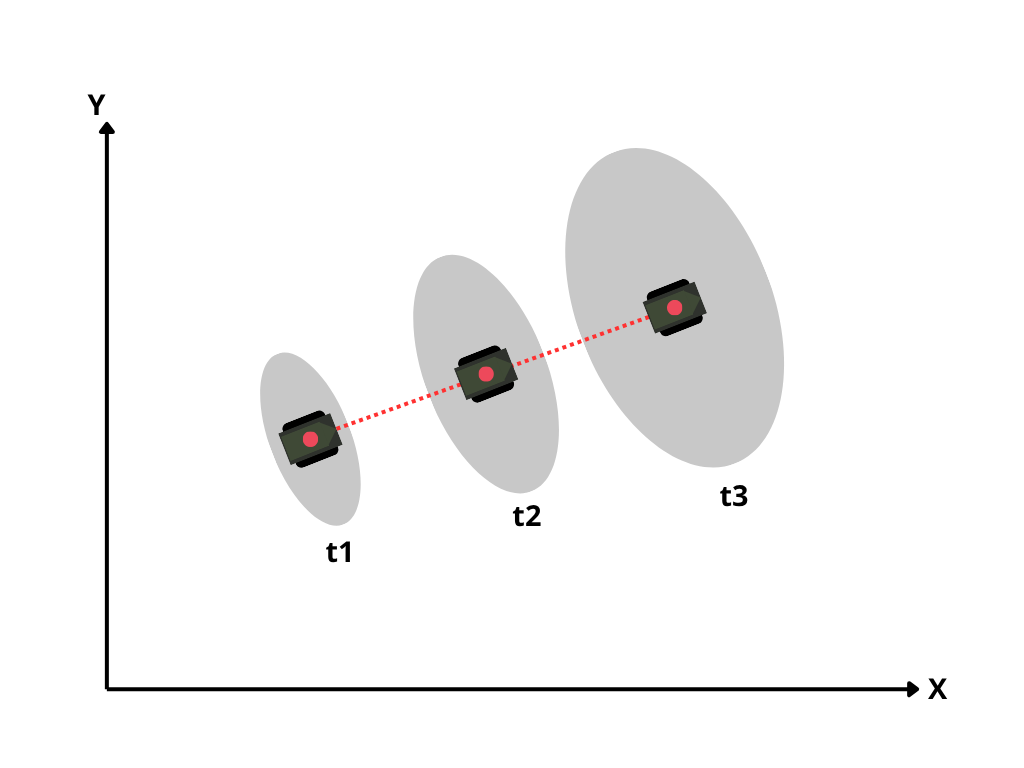
\includegraphics[width=\linewidth]{Figuras/diagrams/OCLUSAO.png}
        \caption{Oclusão: trajetória 1 (predição pura).}
        \label{fig:elipse_crescente_1}
    \end{subfigure}
    \hfill
    % Subfigura C: Crescimento na trajetória 2
    \begin{subfigure}[b]{0.32\textwidth}
        \centering
        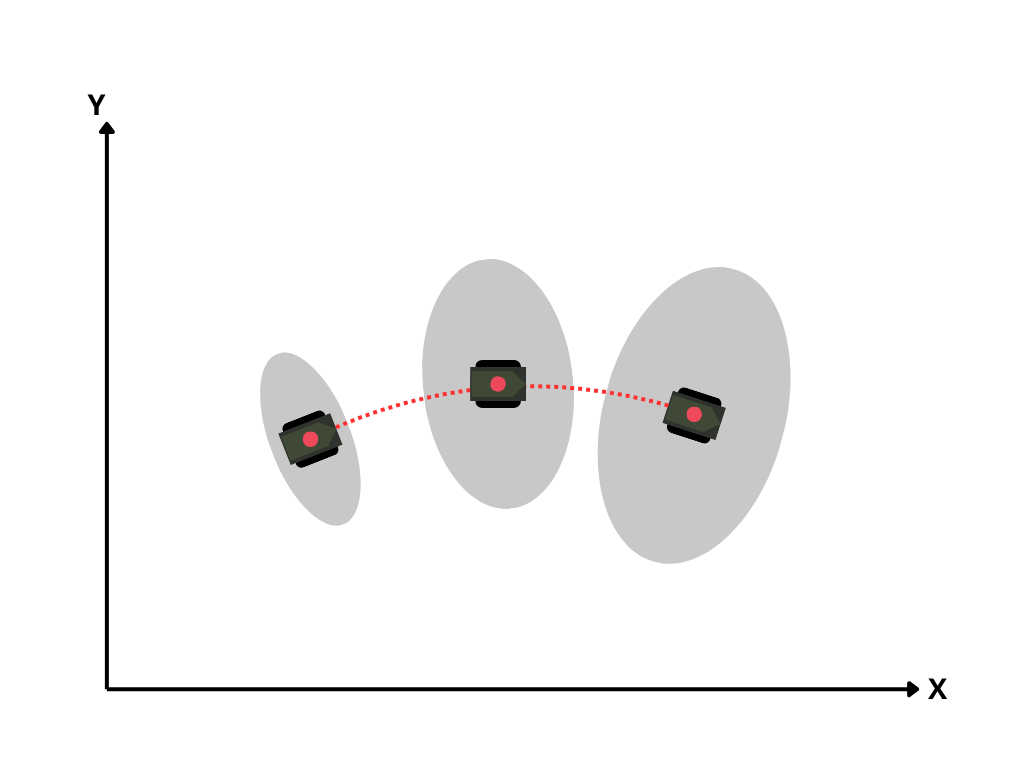
\includegraphics[width=\linewidth]{Figuras/diagrams/OCLUSAO2.png}
        \caption{Oclusão: trajetória 2 (predição pura).}
        \label{fig:elipse_crescente_2}
    \end{subfigure}

    \caption{Representação visual da incerteza do EKF (ROI dinâmica): a elipse em cinza denota a incerteza predita ($\mathbf{P}_{k|k-1}$), enquanto a elipse em verde representa a incerteza atualizada após a correção ($\mathbf{P}_{k|k}$). (a) Regime de operação estável sob observações contínuas; (b) e (c) expansão da incerteza e degradação da precisão decorrentes da supressão das medições (oclusão temporal) em distintos perfis de trajetória.}
    \label{fig:comportamento_elipses}
\end{figure*}